\chapter{Instalasi}
\section{Python 3}
Berikut merupakan tata cara instalasi python 3.
\begin{enumerate}
\item Run program python 3 yang akan di install, ( Dalam hal ini saya melakukan installasi menggunaka anaconda )
\begin{figure}[H]
    \centering
    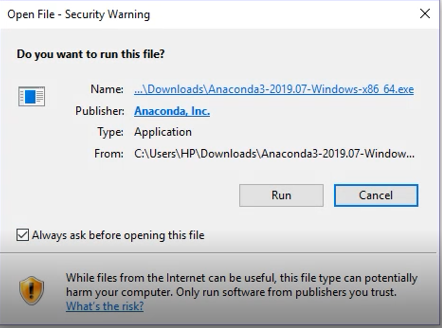
\includegraphics[scale=0.7]{figures/1}
    \label{1}
\end{figure}

\item Klik next saat awal mula installasi
\begin{figure}[H]
    \centering
    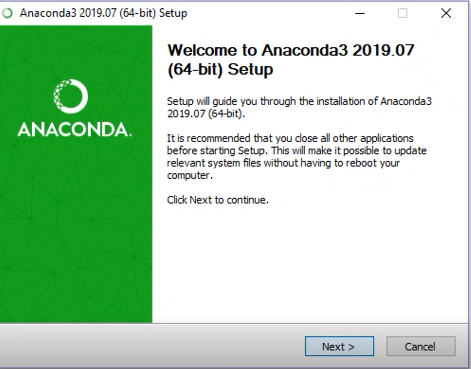
\includegraphics[scale=0.7]{figures/3}
    \label{3}
\end{figure}

\item Klik I agree pada License Agreement jika anda setuju dengan License Agreement tersebut
\begin{figure}[H]
    \centering
    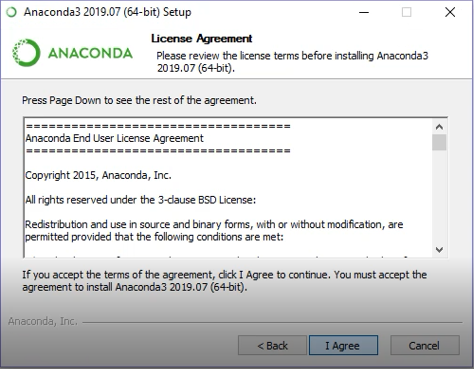
\includegraphics[scale=0.7]{figures/4}
    \label{4}
\end{figure}

\item Tentukan user yang dapat menggunakan aplikasi anaconda nantinya, apakah diperuntukkan untuk semua user atau 1 user saja
\begin{figure}[H]
    \centering
    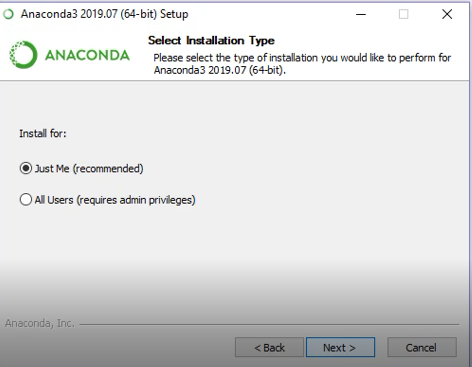
\includegraphics[scale=0.7]{figures/5}
    \label{5}
\end{figure}

\item Melakukan setting opsi tambahan , yaitu menentukan path dan menjadikan anaconda sebagai sebagai aplikasi default python 3.
\begin{figure}[H]
    \centering
    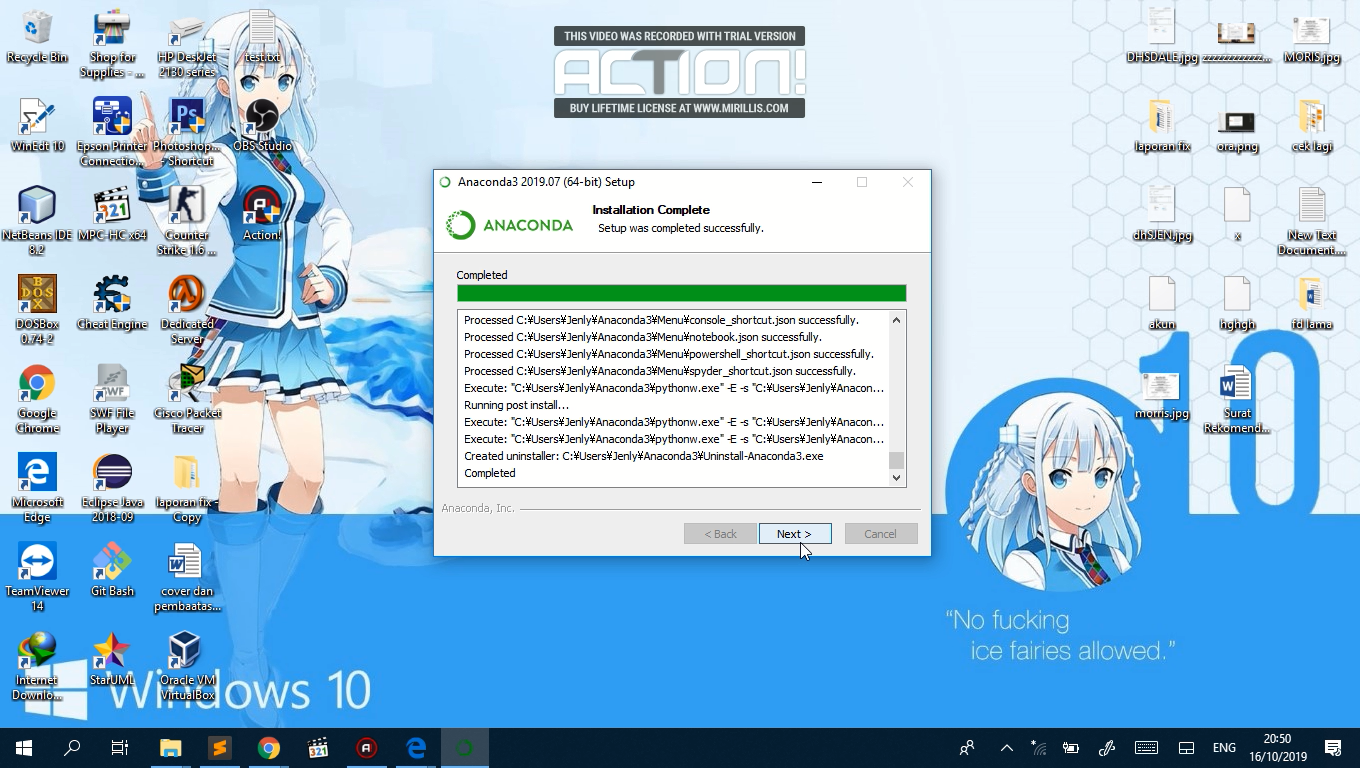
\includegraphics[scale=0.7]{figures/7.png}
    \label{7}
\end{figure}

\item Installasi dilakukan
\begin{figure}[H]
    \centering
    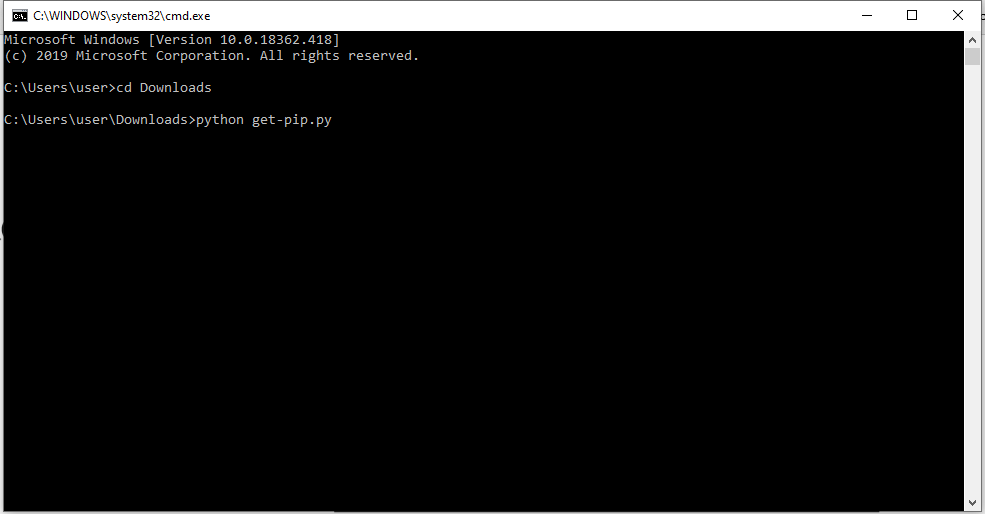
\includegraphics[scale=0.7]{figures/8.png}
    \label{8}
\end{figure}


\item Installasi selesai
\begin{figure}[H]
    \centering
    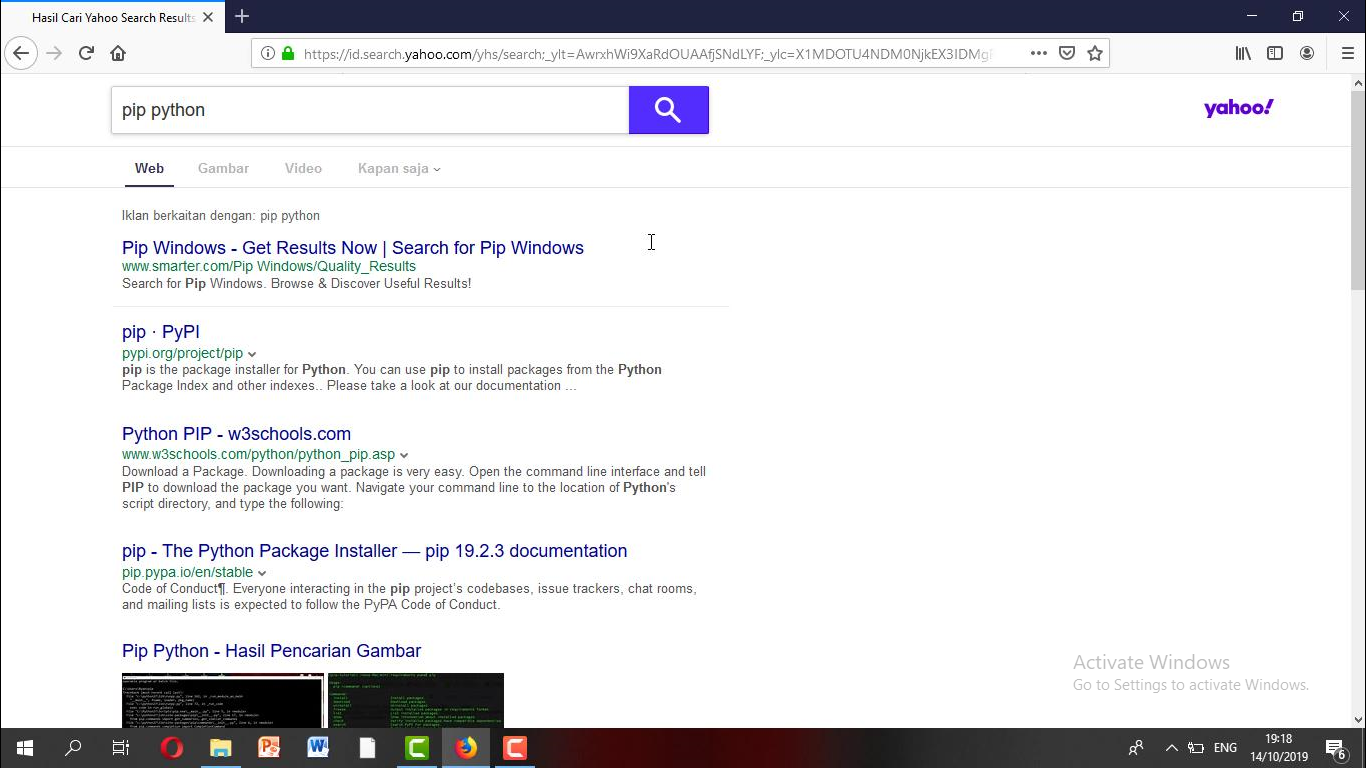
\includegraphics[scale=0.7]{figures/11.png}
    \label{11}
\end{figure}
\end{enumerate}

\section{Pip}
Berikut adalah tata cara melakukan installasi pip
\begin{enumerate}
\item Buka anaconda prompt

\item Jalankan python -m pip install --upgrade pip dan tunggu hingga selesai.
\begin{figure}[H]
    \centering
    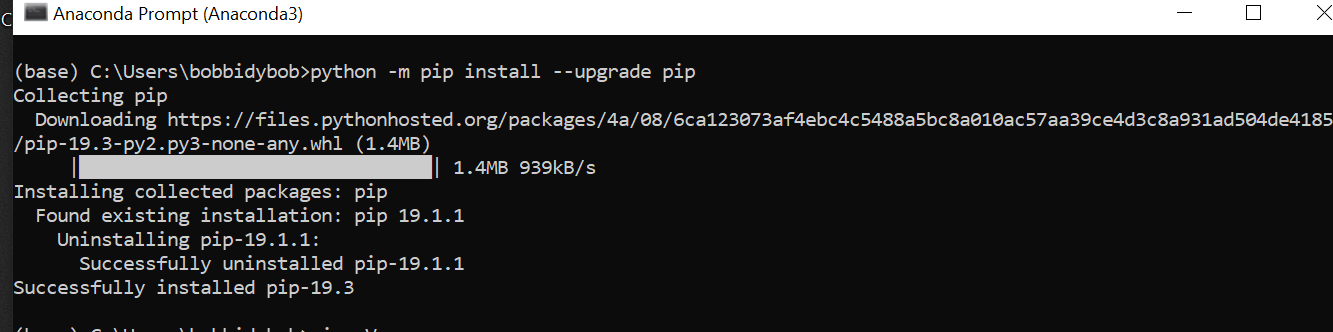
\includegraphics[scale=0.7]{figures/13.png}
    \label{13}
\end{figure}

\item Jika selesai silahkan melakukan pengecekan versi pip yang telah di install dengan pip -V
\begin{figure}[H]
    \centering
    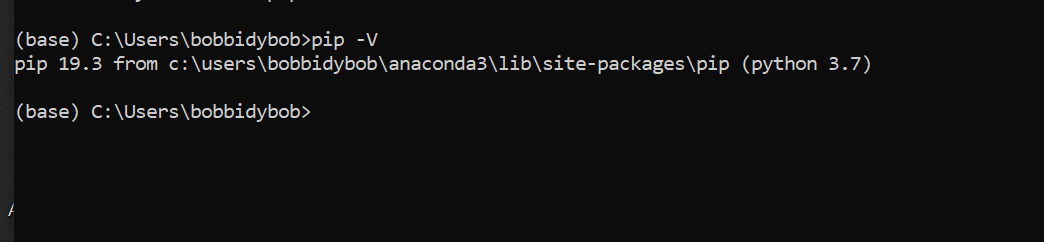
\includegraphics[scale=0.7]{figures/14.png}
    \label{14}
\end{figure}
\end{enumerate}

\section{Setting Environment}
Berikut adalah tata cara Setting Environment.
\begin{enumerate}
\item Buka file explorer
\item Lalu buka properties
\begin{figure}[H]
    \centering
    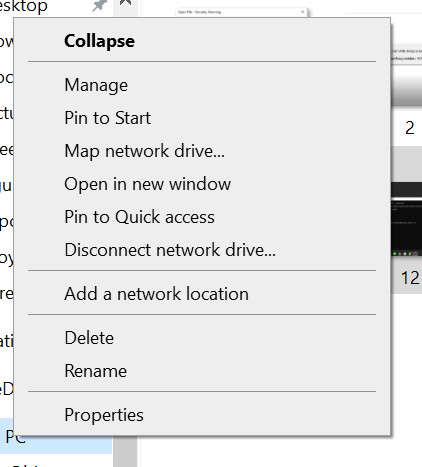
\includegraphics[scale=0.7]{figures/15.png}
    \label{15}
\end{figure}


\item Lalu klik Advance setting
\begin{figure}[H]
    \centering
    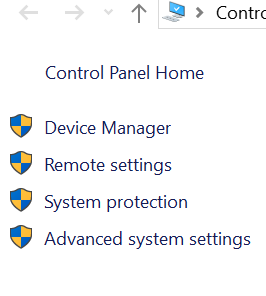
\includegraphics[scale=0.7]{figures/16.png}
    \label{16}
\end{figure}


\item Lalu klik environment variable
\begin{figure}[H]
    \centering
    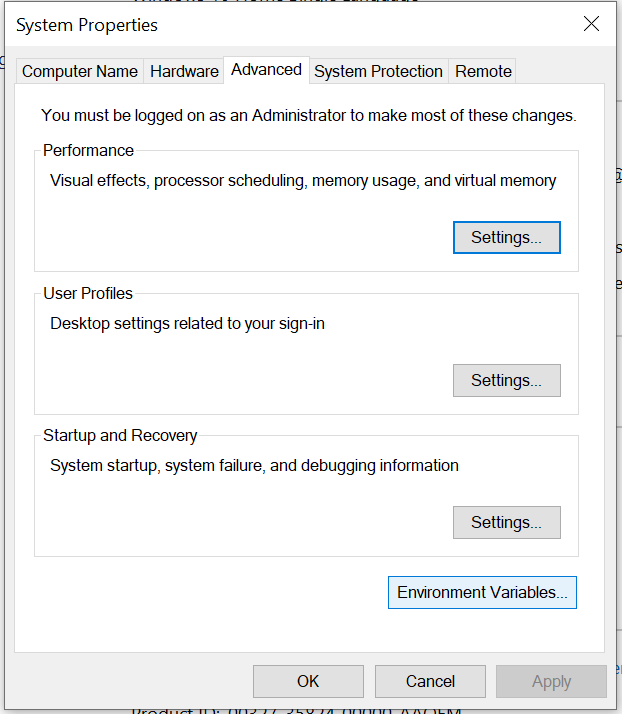
\includegraphics[scale=0.7]{figures/17.png}
    \label{17}
\end{figure}


\item Lalu tambahkan PATH
\begin{figure}[H]
    \centering
    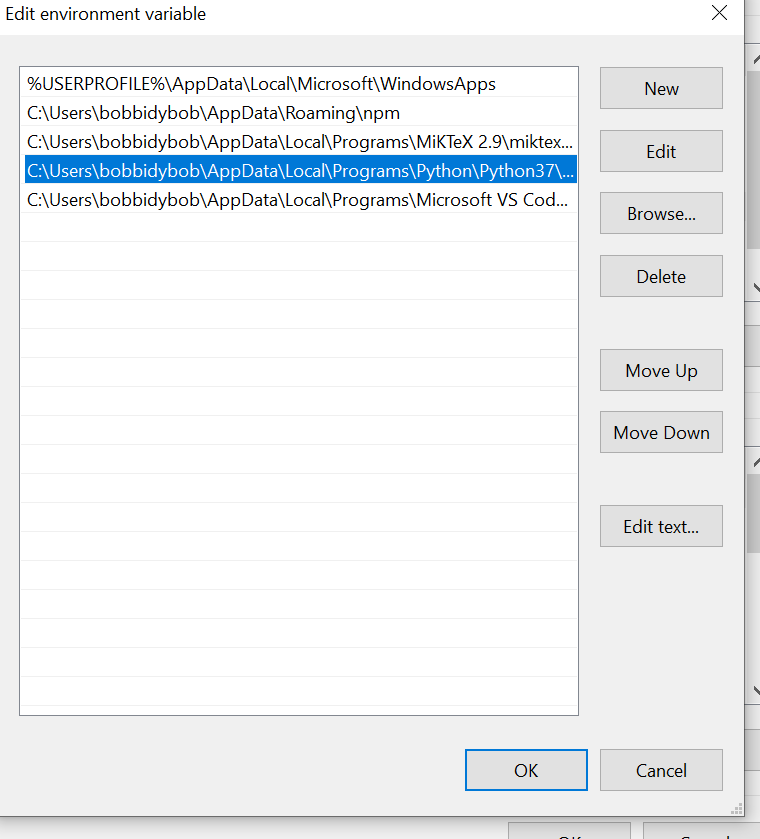
\includegraphics[scale=0.7]{figures/18.png}
    \label{18}
\end{figure}
\end{enumerate}

\section{CLI Melalui Terminal}
Berikut ini cara  mencoba cli melalui terminal 
\begin{enumerate}
\item Buka anaconda prompt
\item lalu ketik python
\item lalu ketik fungsi yang akan dijalankan, pada contoh ini saya akan melakukan fungsi print
\begin{figure}[H]
    \centering
    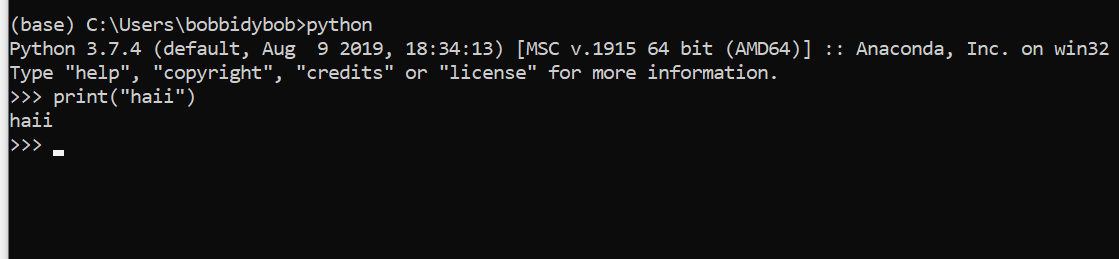
\includegraphics[scale=0.5]{figures/19.png}
    \label{19}
\end{figure}
\end{enumerate}

\section{Anaconda \& Spyder}
Berikut adalah tatacara melakukan update pada anaconda dan spyder.
\begin{enumerate}
\item Buka anaconda prompt

\item Lalu ketikkan conda update anaconda
\begin{figure}[H]
    \centering
    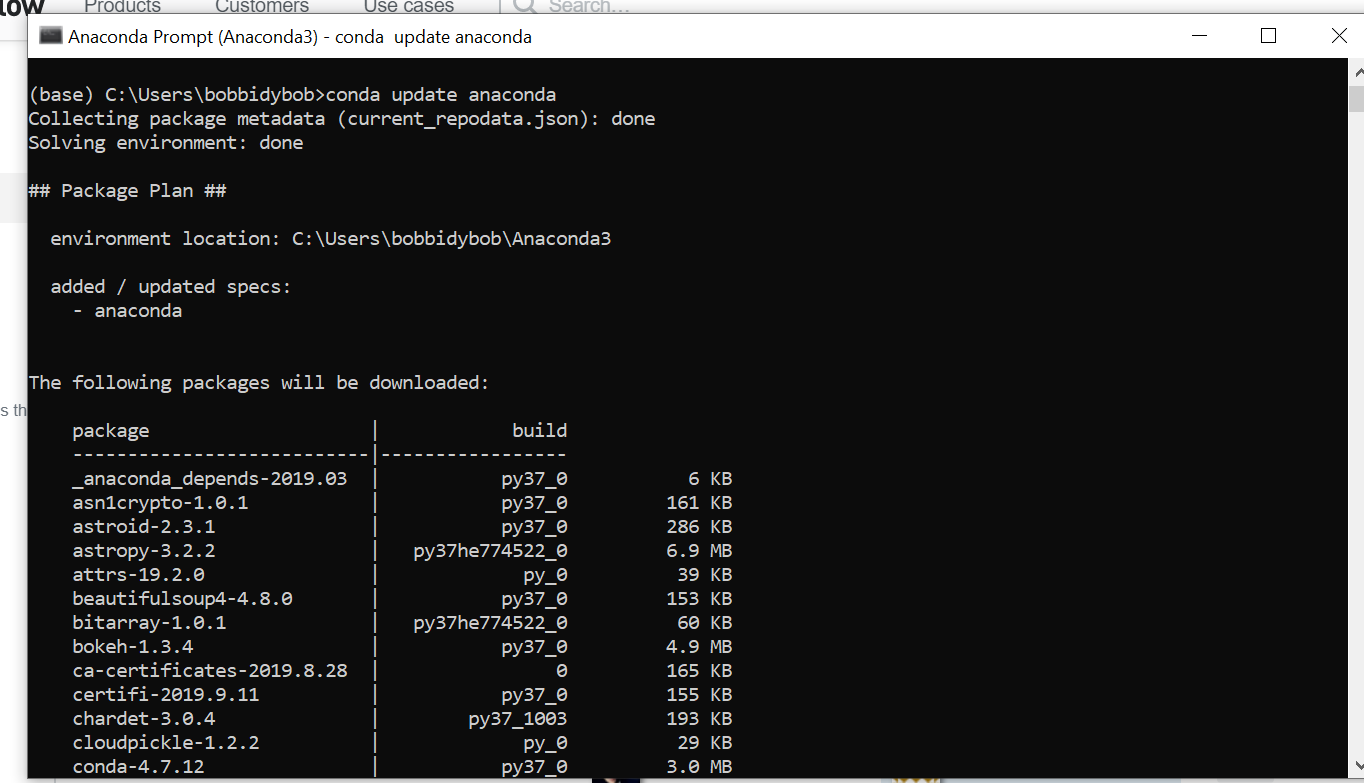
\includegraphics[scale=0.5]{figures/20.png}
    \label{20}
\end{figure}

\item lalu ketik y untuk melanjutkan update
\begin{figure}[H]
    \centering
    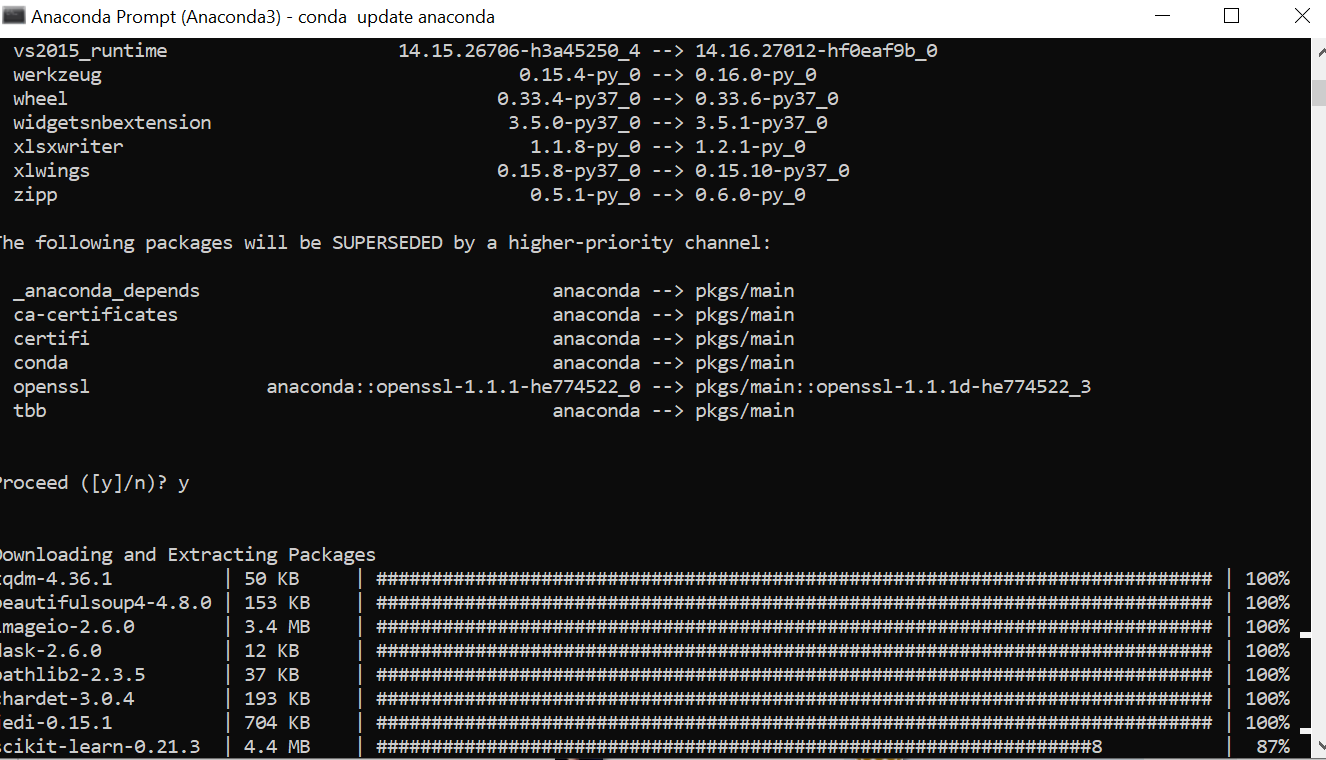
\includegraphics[scale=0.5]{figures/21.png}
    \label{21}
\end{figure}
\item tunggu installasi hingga selesai. (hal yang sama berlaku untuk update spyder)
\end{enumerate}

\section{Hello World}
Berikut adalah cara menjalankan script hello world di spyder
\begin{enumerate}
\item Buka IDE spyder
\item Lalu ketikkan print("hello world")
\begin{figure}[H]
    \centering
    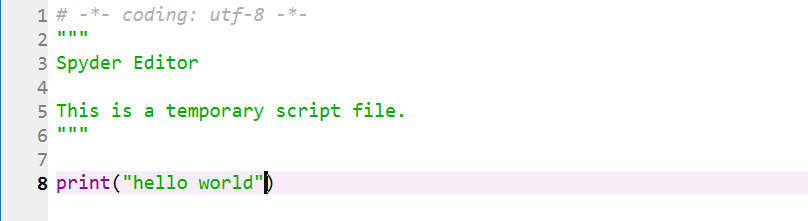
\includegraphics[scale=0.7]{figures/22.png}
    \label{22}
\end{figure}
\item Run program
\item Berikut adalah output dari code yang sudah ditulis
\begin{figure}[H]
    \centering
    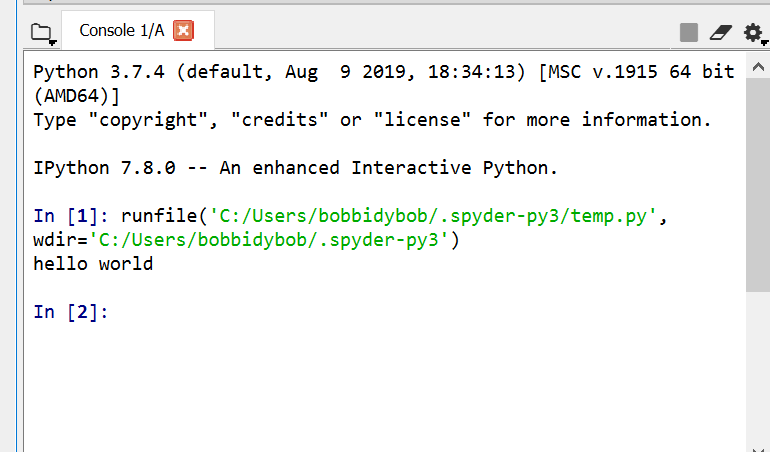
\includegraphics[scale=0.7]{figures/23.png}
    \label{23}
\end{figure}
\end{enumerate}	

\section{Selenium}
Berikut adalah contoh penggunaan selenium
\begin{enumerate}
\item Buka Spyder IDE
\item masukkan kode yang ada pada gambar berikut
\begin{figure}[H]
    \centering
    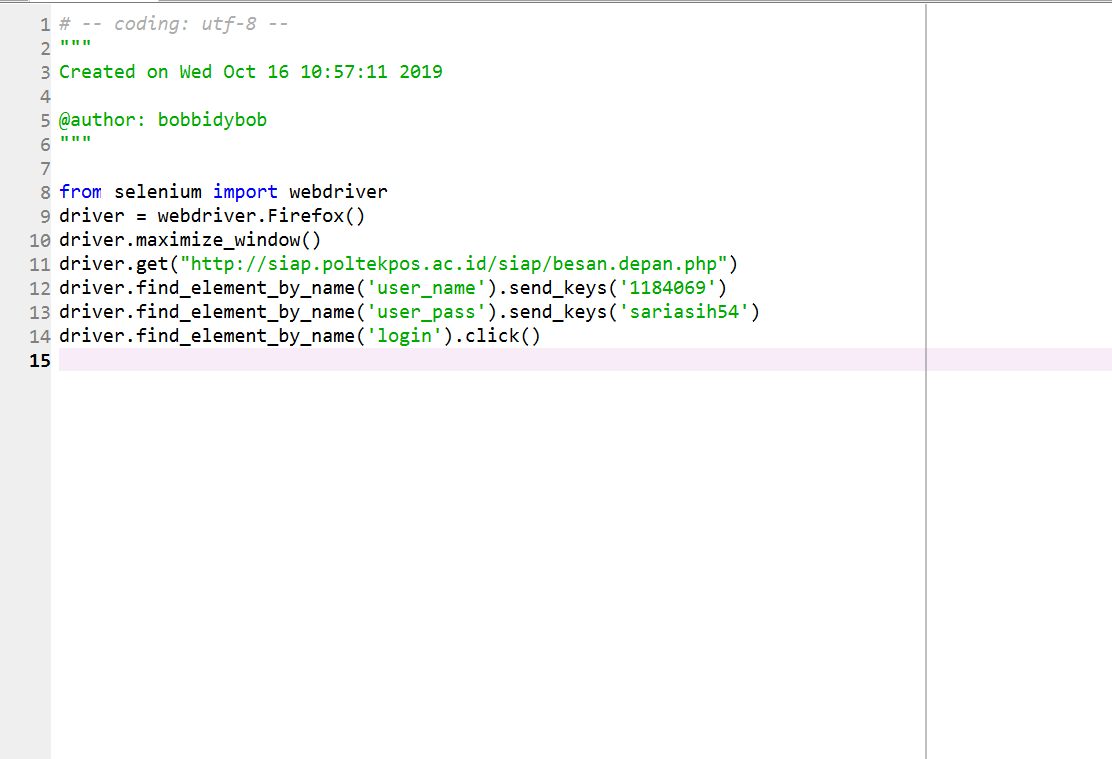
\includegraphics[scale=0.5]{figures/24.png}
    \label{24}
\end{figure}
\item Run program dan lihat apa yang tejadi
\end{enumerate}

\section{Variable Explorer}
Berikut adalah contoh penggunaan selenium
\begin{enumerate}
\item Buka Spyder IDE
\item Masukkan variabel
\begin{figure}[H]
    \centering
    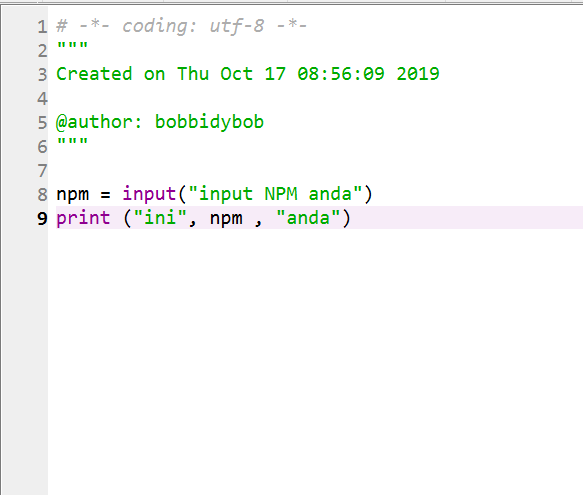
\includegraphics[scale=0.5]{figures/26.png}
    \label{26}
\end{figure}
\item Run program
\item Jika sudah cek variable explorer pada IDE spyder
\begin{figure}[H]
    \centering
    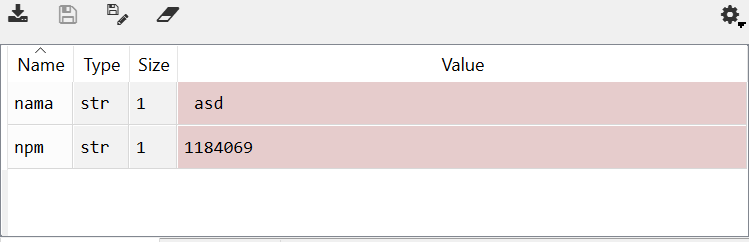
\includegraphics[scale=0.5]{figures/27.png}
    \label{27}
\end{figure}
\end{enumerate}